\upaper{12}{ВСЕЛЕННАЯ ВСЕЛЕННЫХ}
\uminitoc{ПРОСТРАНСТВЕННЫЕ УРОВНИ ГЛАВНОЙ ВСЕЛЕННОЙ}
\uminitoc{ОБЛАСТИ БЕЗУСЛОВНОГО АБСОЛЮТА}
\uminitoc{ВСЕОБЩАЯ ГРАВИТАЦИЯ}
\uminitoc{ПРОСТРАНСТВО И ДВИЖЕНИЕ}
\uminitoc{ПРОСТРАНСТВО И ВРЕМЯ}
\uminitoc{ВСЕОБЩЕЕ СВЕРХУПРАВЛЕНИЕ}
\uminitoc{ЧАСТЬ И ЦЕЛОЕ}
\uminitoc{МАТЕРИЯ, РАЗУМ И ДУХ}
\uminitoc{ЛИЧНОСТНЫЕ РЕАЛЬНОСТИ}
\author{Совершенствователь Мудрости}
\vs p012 0:1 Необъятность обширного творения Всеобщего Отца совершенно недоступна конечному воображению; громадность главной вселенной может поколебать представления даже существ моего порядка. Но смертный разум можно научить многому относительно плана и устройства вселенных; ты можешь узнать кое\hyp{}что об их физической организации и замечательном управлении; ты в состоянии усвоить многое о различных группах разумных существ, населяющих семь сверхвселенных времени и центральную вселенную вечности.
\vs p012 0:2 В принципе, то есть в вечном потенциале, мы представляем материальное творение как бесконечное, ибо Всеобщий Отец действительно бесконечен, но изучая и наблюдая всё материальное творение, мы узнаём, что в любой данный момент времени оно ограниченно, хотя для ваших конечных разумов оно сравнительно беспредельно, практически безгранично.
\vs p012 0:3 Мы убеждены, исходя из изучения физических законов и наблюдений за звёздными мирами, что бесконечный Создатель ещё не проявлен в полноте космического выражения, что б\'ольшая часть космического потенциала Бесконечного всё ещё заключена в нём самом и не раскрыта. Созданным существам главная вселенная может показаться почти бесконечной, но она ещё далека от завершения; материальное творение по\hyp{}прежнему имеет физические пределы, и эмпирическое откровение вечного замысла всё ещё продолжается.
\usection{ПРОСТРАНСТВЕННЫЕ УРОВНИ ГЛАВНОЙ ВСЕЛЕННОЙ}
\vs p012 1:1 Вселенная вселенных --- это не бесконечная плоскость, безграничный куб или беспредельный круг; она несомненно имеет размеры. Законы физической организации и управления неопровержимо доказывают, что всё огромное скопление силы\hyp{}энергии и материи\hyp{}мощи функционирует в конечном счёте как пространственная\fnst{Или <<космическая>> (англ. space).} единица, как организованное и согласованное целое. Наблюдаемое поведение материального творения свидетельствует о наличии определённых пределов в физической вселенной. Окончательным доказательством как кругообразности, так и ограниченности вселенной служит хорошо известный нам факт, что все формы основной энергии вечно обращаются по изогнутой траектории пространственных уровней главной вселенной, подчиняясь непрекращающемуся и абсолютному притяжению Райской гравитации.
\vs p012 1:2 Последовательные пространственные уровни главной вселенной составляют основные подразделения насыщенного пространства --- всё творение, организованное и частично заселённое или ещё не организованное и не заселённое. Если бы главная вселенная не являлась последовательностью эллиптических пространственных уровней с уменьшенным сопротивлением движению, чередующихся с зонами относительного покоя, мы полагаем, что можно было бы наблюдать, как некоторые из космических энергий вылетают на бесконечное расстояние по прямолинейным траекториям в безбрежную необъятность космоса; но мы никогда не встречали силу, энергию или материю, ведущие себя подобным образом; они вечно кружатся, всегда обращаясь по следам великих космических контуров.
\vs p012 1:3 \pc Продвигаясь от Рая наружу через горизонтальное протяжение насыщенного пространства, главная вселенная предстаёт в виде шести концентрических эллипсов --- пространственных уровней, окружающих центральный Остров:
\vs p012 1:4 \li{1.}Центральная Вселенная --- Хавона.
\vs p012 1:5 \li{2.}Семь сверхвселенных.
\vs p012 1:6 \li{3.}Первый внешний пространственный уровень.
\vs p012 1:7 \li{4.}Второй внешний пространственный уровень.
\vs p012 1:8 \li{5.}Третий внешний пространственный уровень.
\vs p012 1:9 \li{6.}Четвёртый и самый дальний внешний пространственный уровень.
\vs p012 1:10 \pc \bibemph{Хавона,} центральная вселенная, не является творением времени; она представляет собой вечное существование. Эта не имеющая начала и конца вселенная состоит из миллиарда сфер высочайшего совершенства и окружена огромными тёмными гравитационными телами. В центре Хавоны находится неподвижный и абсолютно устойчивый Остров Рай, окружённый 21 спутником. Из\hyp{}за огромных масс окружающих тёмных гравитационных тел, находящихся у края центральной вселенной, общая масса этого центрального творения намного превышает полную известную массу всех семи секторов большой вселенной.
\vs p012 1:11 \pc \bibemph{Система Рай\hyp{}Хавона,} вечная вселенная, окружающая вечный Остров, составляет совершенное и вечное ядро главной вселенной; все семь сверхвселенных и все области внешнего пространства обращаются по установленным орбитам вокруг гигантского центрального скопления спутников Рая и сфер Хавоны.
\vs p012 1:12 Семь сверхвселенных не являются первичными физическими структурами; нигде их границы не разделяют семейство туманностей\fnst{В начале XX века галактики назывались <<туманностями>>.}, как не пересекают они ни одну локальную вселенную --- основную единицу творения. Каждая сверхвселенная --- это просто географическое пространственное объединение примерно одной седьмой части организованного и частично заселённого пост\hyp{}Хавонского творения, и все они примерно равны по числу входящих в них локальных вселенных и по занимаемому пространству. \bibemph{Небадон,} ваша локальная вселенная, --- одно из новых творений в \bibemph{Орвонтоне,} седьмой сверхвселенной.
\vs p012 1:13 \bibemph{Большая Вселенная} --- это существующее в настоящее время организованное и обитаемое творение. Она состоит из семи сверхвселенных, совокупный эволюционный потенциал которых составляет около семи триллионов обитаемых планет, не считая вечных сфер центрального творения. Но эта предварительная оценка не учитывает ни архитектурных административных сфер, ни отдалённых групп неорганизованных вселенных. Нынешний зубчатый край большой вселенной, её неровная и незавершённая периферия, вместе с чрезвычайно неустойчивым состоянием всего астрономического участка, наводят наших исследователей звёзд на мысль, что даже семь сверхвселенных пока ещё не завершены. Двигаясь изнутри, от божественного центра наружу в любом направлении, мы, в конце концов, приходим к внешним пределам организованного и обитаемого творения; мы подходим к внешним пределам большой вселенной. И именно у такого внешнего рубежа, в далёком уголке этого величественного творения, ваша локальная вселенная продолжает своё богатое событиями существование.
\vs p012 1:14 \bibemph{Внешние пространственные уровни}. Далеко в космосе, на огромном расстоянии от семи обитаемых сверхвселенных, собираются огромные и невероятно колоссальные контуры силы и материализующейся энергии. Между энергетическими контурами семи сверхвселенных и этим гигантским внешним поясом силовой активности находится пространственная зона относительного покоя, которая изменяется по ширине, но в среднем составляет около 400\,000 световых лет. Эти пространственные зоны свободны от звёздной пыли --- космического тумана. Наши исследователи этих явлений пребывают в сомнении относительно точного статуса сил пространства, существующих в этой зоне относительного покоя, окружающей семь сверхвселенных. Но на расстоянии примерно в 500\,000 световых лет от периферии нынешней большой вселенной мы наблюдаем начало зоны невероятной энергетической активности, объём и интенсивность которой увеличивается на протяжении более чем 25\,000\,000 световых лет. Эти гигантские колёса возбуждающих сил расположены в первом внешнем пространственном уровне --- непрерывном поясе космической активности, окружающем всё известное, организованное и обитаемое творение.
\vs p012 1:15 Ещё б\'ольшая активность происходит за пределами этих областей, ибо физики Уверсы обнаружили ранние свидетельства проявления силы на расстоянии более 50\,000\,000 световых лет от самых отдалённых областей этих явлений в первом внешнем пространственном уровне. Эта активность, несомненно, предвещает организацию материальных творений второго внешнего пространственного уровня главной вселенной.
\vs p012 1:16 Центральная вселенная есть творение вечности; семь сверхвселенных --- творения времени; четыре внешних пространственных уровня, несомненно, предназначены для возникновения\hyp{}эволюции предельности творения. И есть те, кто утверждают, что Бесконечный никогда не может достичь полного выражения, иначе как в бесконечности; и поэтому они постулируют дополнительное и нераскрытое творение за пределами четвёртого и самого дальнего пространственного уровня --- возможность постоянно расширяющейся, никогда не кончающейся вселенной бесконечности. Теоретически мы не знаем, как ограничить бесконечность Создателя или потенциальную бесконечность творения, но в том виде, как она существует и управляется, мы рассматриваем главную вселенную как имеющую пределы, как определённым образом разграниченную и окаймлённую на своих внешних границах открытым пространством.
\usection{ОБЛАСТИ БЕЗУСЛОВНОГО АБСОЛЮТА}
\vs p012 2:1 Когда астрономы Урантии всматриваются в свои всё более мощные телескопы в таинственные дали внешнего пространства и видят там удивительную эволюцию почти бесчисленных физических вселенных, им следует осознать, что перед их взором предстаёт могущественная реализация непостижимых планов Архитекторов Главной Вселенной. Конечно, у нас есть свидетельства, которые наводят на мысль о присутствии определённых Райских личностных влияний --- здесь и там --- по всем обширным энергетическим проявлениям, которые в настоящее время характерны для этих внешних областей, но если смотреть шире, области пространства, простирающиеся за внешними границами семи сверхвселенных, обычно признаются как составляющие владения Безусловного Абсолюта.
\vs p012 2:2 Хотя невооружённым глазом человека можно увидеть только две или три туманности за пределами сверхвселенной Орвонтон\fnst{То есть <<галактики>>. Невооружённому глазу в северном полушарии доступны только две галактики: М31 Туманность Андромеды и М33 в созвездии Треугольника. Большое и Малое Магеллановы Облака видны только в южном полушарии и считаются спутниками нашей Галактики. Отсюда следует, что галактика Туманность Андромеды находится \bibemph{за пределами сверхвселенной Орвонтон}, см.\,\bibref[15:4.7]{p015 4:7}.}, ваши телескопы буквально раскрывают миллионы и миллионы этих физических вселенных, находящихся в процессе формирования. Большинство звёздных миров, визуально доступных наблюдению в ваши современные телескопы, находятся в Орвонтоне, но с помощью фотографической техники более крупные телескопы проникают далеко за пределы большой вселенной в области внешнего пространства, где бесчисленные вселенные находятся в процессе формирования. И ещё многие миллионы вселенных остаются за пределами досягаемости ваших нынешних инструментов.\tunemarkup{pictures}{\begin{figure}[H]\centering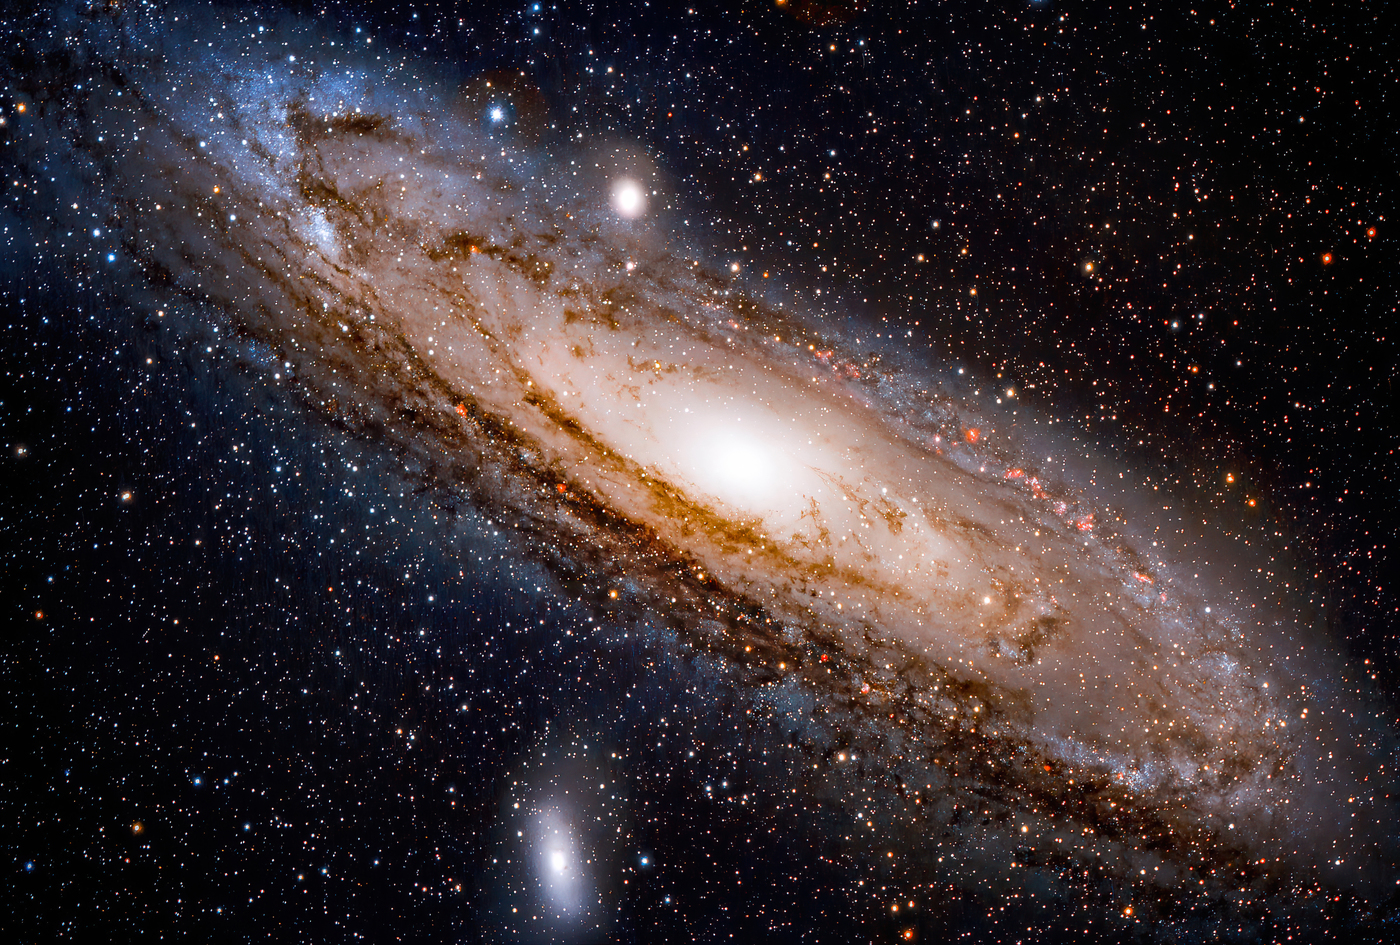
\includegraphics[width=0.99\columnwidth]{images/M31.jpg}\caption{Галактика Туманность Андромеды (М31)}\end{figure}}
\vs p012 2:3 В недалёком будущем\fnst{Написано в 30\hyp{}е года XX века.} новые телескопы откроют удивлённому взору астрономов Урантии не менее 375\,000\,000 новых галактик в отдалённых областях внешнего пространства. В то же время эти более мощные телескопы покажут, что многие островные вселенные\fnst{Так раньше назывались галактики (англ. island universes).}, ранее считавшиеся находящимися во внешнем пространстве, на самом деле являются частью галактической системы Орвонтон. Семь сверхвселенных всё ещё растут; периферия каждой из них постепенно расширяется; новые туманности постоянно стабилизируются и организуются; и некоторые из туманностей, которые астрономы Урантии считают внегалактическими, на самом деле находятся на окраине Орвонтона и путешествуют вместе с нами\fnst{Возможно, что речь идёт о Большом и Малом Магеллановых Облаках.}.
\vs p012 2:4 \pc Астрономы [star students] Уверсы отмечают, что большая вселенная окружена предшественниками ряда звёздных и планетарных скоплений, которые полностью окружают нынешнее обитаемое творение в виде концентрических колец внешних многочисленных вселенных. Физики Уверсы подсчитали, что энергия и материя этих внешних и неизведанных областей уже во много раз превышают общую материальную массу и энергетический заряд, заключенный во всех семи сверхвселенных. Мы знаем, что превращение космической силы в этих внешних пространственных уровнях является функцией Райских организаторов силы. Мы также знаем, что эти силы предшествуют тем физическим энергиям, которые в настоящее время активируют большую вселенную. Однако управляющие энергией Орвонтона не имеют никакого отношения к этим удалённым мирам, а движения энергии в них не связаны явным образом с контурами мощи организованных и обитаемых творений.\tunemarkup{pictures}{\begin{figure}[H]\centering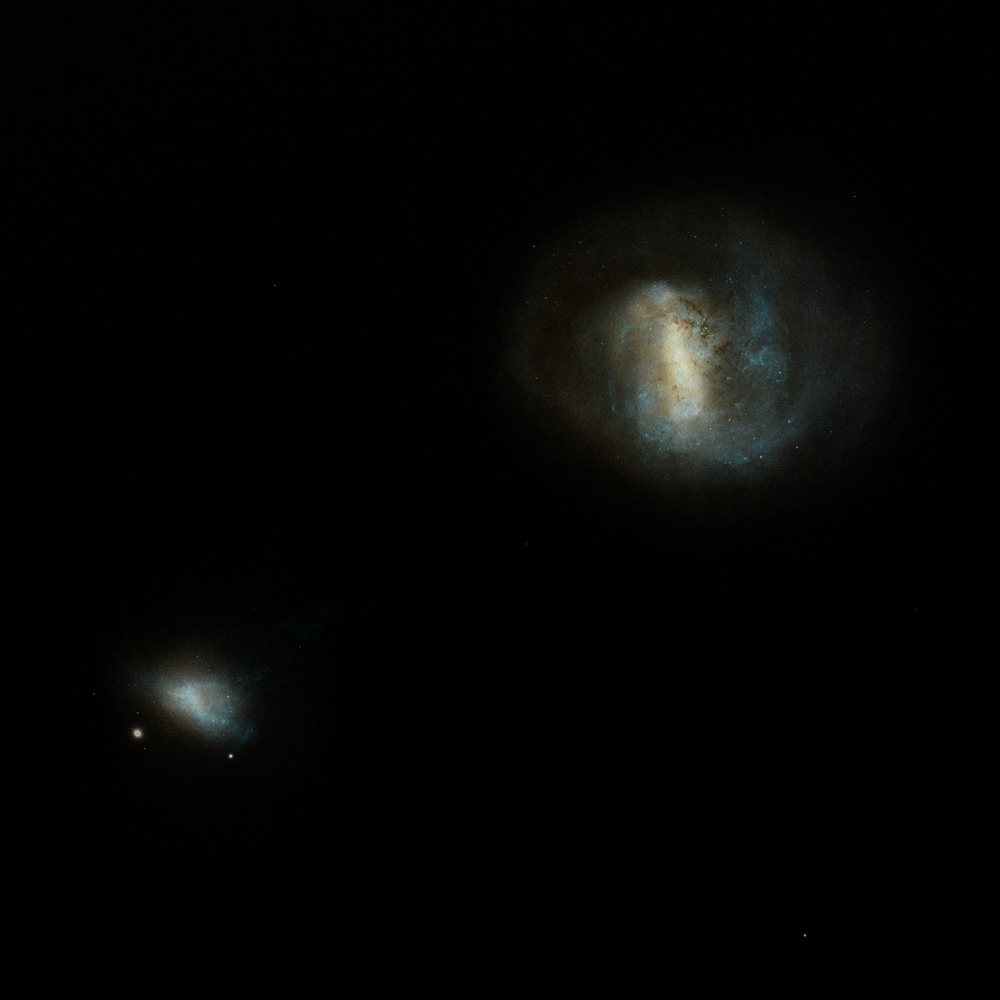
\includegraphics[width=0.99\columnwidth]{images/LMC.jpg}\caption{Большое и Малое Магеллановы Облака}\end{figure}}
\vs p012 2:5 \pc Мы очень мало знаем о значении этих грандиозных явлений внешнего пространство. Ещё более великое творение будущего находится в процессе формирования. Мы наблюдаем его необъятность, мы можем различать его протяжённость и ощущать его величественные размеры, но в остальном мы знаем об этих сферах немногим больше, чем астрономы Урантии. Насколько нам известно, в этом внешнем кольце туманностей, солнц и планет нет материальных существ вроде людей, ангелов или других духовных созданий. Эта далёкая область находится вне юрисдикции и управления правительств сверхвселенных.
\vs p012 2:6 Повсюду в Орвонтоне считается, что имеет место процесс творения нового типа, тип вселенных, которому суждено стать ареной будущих действий собирающегося Корпуса Завершения; и если наши предположения верны, то бесконечное будущее может принести всем вам те же захватывающие дух зрелища, которые бесконечное прошлое содержало для ваших старших [seniors] и предшественников.
\usection{ВСЕОБЩАЯ ГРАВИТАЦИЯ}
\vs p012 3:1 
\vs p012 3:2 
\vs p012 3:3 
\vs p012 3:4 
\vs p012 3:5 
\vs p012 3:6 \pc 
\vs p012 3:7 
\vs p012 3:8 
\vs p012 3:9 
\vs p012 3:10 
\vs p012 3:11 
\vs p012 3:12 \pc 
\usection{ПРОСТРАНСТВО И ДВИЖЕНИЕ}
\vs p012 4:1 
\vs p012 4:2 
\vs p012 4:3 
\vs p012 4:4 
\vs p012 4:5 
\vs p012 4:6 \pc 
\vs p012 4:7 \pc 
\vs p012 4:8 
\vs p012 4:9 
\vs p012 4:10 
\vs p012 4:11 
\vs p012 4:12 \pc 
\vs p012 4:13 
\vs p012 4:14 \pc 
\vs p012 4:15 
\vs p012 4:16 
\usection{ПРОСТРАНСТВО И ВРЕМЯ}
\vs p012 5:1 
\vs p012 5:2 
\vs p012 5:3 \pc 
\vs p012 5:4 
\vs p012 5:5 \pc 
\vs p012 5:6 \pc 
\vs p012 5:7 
\vs p012 5:8 
\vs p012 5:9 
\vs p012 5:10 \pc 
\vs p012 5:11 
\usection{ВСЕОБЩЕЕ СВЕРХУПРАВЛЕНИЕ}
\vs p012 6:1 
\vs p012 6:2 
\vs p012 6:3 
\vs p012 6:4 
\vs p012 6:5 
\vs p012 6:6 \pc 
\vs p012 6:7 
\vs p012 6:8 \pc 
\vs p012 6:9 
\vs p012 6:10 
\vs p012 6:11 
\vs p012 6:12 
\vs p012 6:13 \pc 
\usection{ЧАСТЬ И ЦЕЛОЕ}
\vs p012 7:1 
\vs p012 7:2 \pc 
\vs p012 7:3 
\vs p012 7:4 
\vs p012 7:5 
\vs p012 7:6 
\vs p012 7:7 \pc 
\vs p012 7:8 
\vs p012 7:9 
\vs p012 7:10 
\vs p012 7:11 
\vs p012 7:12 \pc 
\vs p012 7:13 \pc 
\vs p012 7:14 
\usection{МАТЕРИЯ, РАЗУМ И ДУХ}
\vs p012 8:1 
\vs p012 8:2 \pc 
\vs p012 8:3 
\vs p012 8:4 \pc 
\vs p012 8:5 
\vs p012 8:6 \pc 
\vs p012 8:7 
\vs p012 8:8 
\vs p012 8:9 \pc 
\vs p012 8:10 
\vs p012 8:11 
\vs p012 8:12 
\vs p012 8:13 \pc 
\vs p012 8:14 \pc 
\vs p012 8:15 
\vs p012 8:16 
\usection{ЛИЧНОСТНЫЕ РЕАЛЬНОСТИ}
\vs p012 9:1 
\vs p012 9:2 \pc 
\vs p012 9:3 
\vs p012 9:4 
\vs p012 9:5 
\vs p012 9:6 \pc 
\vsetoff
\vs p012 9:7 
\quizlink
